\chapter{Discussion}
\label{ch:discussion}

%\section{Neutron Stars}
%\label{sec:dis_ns}
%The paths followed by neutron stars in the \ac{PCC}~diagram given in Fig.~\ref{fig:pc_all_ns} reveal some interesting points. Firstly, the tracks trace out an elliptical shape, similar to the paths black holes showed in \citet{heil2015power}. Secondly, while the tracks follow a tight track towards the bottom right, a large degree of scatter is found in the left part of the diagram. Thirdly, as visible in appendix~\ref{ch:pccds}, few sources show a complete oval track across the full \ac{PCC}~diagram, but more often remain confined to particular sections. In order to understand the evolution of neutron stars in the \ac{PCC}~diagram, an in-depth look at the general trend in power spectral properties is warranted. Both Fig.~\ref{fig:ps_overview} and appendix~\ref{ch:psds} show the evolution of power spectra throughout the \ac{PCC}~diagram, with appendix~\ref{ch:psds} containing additional power spectra. Similar to the work done previously in \citet{heil2015power} for black hole systems, the following paragraphs describe the observed trends per spectral state. To help with placing neutron stars in the context of black holes, the choice is made to describe the neutron star evolution in terms of the corresponding black hole states. 
%
%\paragraph{Hard State} With the hard state ranging from a hue angle of approximately 340$^\circ$--140$^\circ$, neutron star power spectra commonly are broad and flat (appendix~\ref{ch:psds}; Figs. \ref{fig:ps_0_20}-\ref{fig:ps_120_140}). The flat power spectra result in \ac{PCC} values tending to be located around (1,1) as seen in Fig.~\ref{fig:pc_hue_bins}. Though some overlap occurs between the hard and the soft state in the \ac{PCC}~diagram, a distinction between both states can be made using the energy spectral hardness or the total \ac{RMS} variability \citep{heil2015power}. Neutron star power spectra and black hole power spectra are broadly comparable in behaviour at these hues, though errors tend to be smaller in black hole systems. An interesting point is that black hole systems show a relatively well-defined track in the \ac{PCC}~diagram in this state, similar to the neutron stars, as can be seen in Fig.~\ref{fig:ns_bh}. The relative narrowness of the track in comparison to other states seems however to be stronger in neutron stars. 
%
%\paragraph{Hard-Intermediate State} Transitioning from the hard state at approximately 140$^\circ$ up to about 220$^\circ$, a broad 'hump' gradually starts to emerge at the central frequencies of neutron star power spectra, slowly growing and shifting to higher frequencies (appendix~\ref{ch:psds}; Figs. \ref{fig:ps_140_160}-\ref{fig:ps_200_220}). While black hole power spectra typically show strong type~C \QPOs at these hue values \citep{heil2015power}, similar \QPOs in neutron stars tend to be less prominent in comparison to the overall power. Most noticeable are the low frequency \QPOs appearing in the power spectra of for instance XTE~J1701-462 and Cyg~X-2. \citet{heil2015inclination} showed that removing the type~C \QPOs in this state for black hole systems significantly reduced the scatter in the softer hard-intermediate states. Potentially a similar effect would be expected with neutron stars, whereby \QPOs partially contribute to the scatter observed at the lower apex. The role of \QPOs in power colours is discussed further in section~\ref{sec:dis_incl}, coupling the effects of \QPOs on power colours with possible \ac{QPO} origins.
%
%\paragraph{Soft-Intermediate State} Ranging between approximately 220$^\circ$--300$^\circ$, neutron star power spectra show increasingly steeper spectra at high frequencies, with additional power emerging at lower frequencies (appendix~\ref{ch:psds}; Figs. \ref{fig:ps_220_240}-\ref{fig:ps_280_300}). Together with the soft state, observations show a large degree of variability in the power spectra, with sudden troughs and peaks appearing from one observation to the next. While black holes typically show strong variability rapidly reducing in power at high frequencies in this state, neutron stars seem to show only the slightest drop in power at these high frequencies. Extending neutron star power spectra out to higher frequencies would show a rapid drop at kHz frequencies \citep{kleinwolt}, but with power colours only probing lower frequencies this plays no role in the analysis. Similar to the black holes, neutron stars show a large degree of scatter in the \ac{PCC}~diagram in this state.
%
%\paragraph{Soft State} The final canonical spectral state runs from approximately 300$^\circ$ to 20$^\circ$. Coupled with a high count rate in comparison to observations in the hard state, neutron star power spectra show an increasing likeness to black hole power spectra. Power spectra flatten out fairly rapidly, with power falling away at the highest frequencies (appendix~\ref{ch:psds}; Figs. \ref{fig:ps_300_320}-\ref{fig:ps_340_360}). \\
%
%\subsection{Spectral States}
%\label{sec:dis_states}
%While the evolution of neutron stars across the \ac{PCC}~diagram can be understood in terms of power spectral evolution, the strength of power colours lies in their ability to describe the spectral state evolution of black holes. Establishing such a relation for neutron stars spectral states would allow neutron star and black systems with similar states to be compared, and therefore is the primary aspect for which neutron star power colours should be tested. While black holes shows a relation between spectral states and their \ac{PCC} track, this relationship does not necessarily have to hold for neutron stars. Commonly spectral states in neutron stars are defined on basis of \ac{ECC}~diagrams. Similar to power colours, the ratios reduce the influence of shifting energy dependent features and provide a means of classifying sources. Difficulties arise however upon comparing various sources with each other, where Z-shaped tracks can cause atoll sources to be classified as Z sources \citep[see][]{muno2002z,gierlinski2002comment}. As seen in Fig.~\ref{fig:cc} for Aql~X-1, several of these states can be linked to directly to the states exhibited by black holes. A clear relationship can be established between the \ac{EIS} and the hard state in the black holes systems as noted by \citet{van1994similarities}. While individual banana states do not show distinct paths in the \ac{PCC}~diagram, the banana state as a whole is unambiguously related to the soft states of black hole systems. With neutron stars commonly transitioning quickly through the lower apex in the \ac{PCC}~diagram, it is difficult to link the \ac{IS} to the intermediate states of black hole systems. Tentative links emerge between these states while looking at \acp{PCC} with errors slightly larger than the $3\sigma$ cut applied to the \ac{PCC}~diagrams.\\
%
%Inspecting the combination of \ac{PCC}, \ac{HH} and \ac{HI}~diagrams provides an alternative way to test the link between spectral states and position in the \ac{PCC}~diagram. Tests show an excellent agreement between for instance high intensity observations with a high hardness and the position in the \ac{PCC}~diagram, located in the area corresponding to hard states in black holes. Such relationships break down however for two objects -- Cir~X-1 and EXO~0748-676. Since these two sources display differing power colour behaviours by which potential misclassification of spectral states could arise, they were removed from the general overview of neutrons star power colours seen in Fig.~\ref{fig:pc_all_ns}, and from further analysis. A full discussion on the nature of these sources is given in section~\ref{sec:oddballs}.\\
%
%%==========================================================================
%\section{Neutron Stars \& Black Holes}
%\label{sec:dis_nsbh}
%Fig.~\ref{fig:ns_bh} shows the striking similarity between neutron star \ac{PCC} tracks and black hole ones, confirming the power spectral relationships explored in previous studies \citep[e.g.][]{wijnands1999broadband,sunyaev2000fourier,klein2008identification}. While specific power spectral features vary between neutron stars and black holes, the congruity in \ac{PCC}~paths show the broadband components under 16~Hz change in a similar fashion regardless of the compact object.\\
%
%The second noticeable feature is the clear distinction between both types of objects in the upper-right part of the \ac{PCC}~diagram. Originating from the broad component present in neutron star power spectra, which is absent from black hole power spectra \citep[see][]{sunyaev2000fourier}, it provides an excellent means of distinguishing black holes and neutron stars in a model-independent way. As explored in earlier studies, the broader power spectra of neutron stars exhibit similar features to black hole power spectra at lower frequencies \citep{klein2008identification}. Shifting the power colour frequency bands up for neutron stars might allow for a more accurate comparison to be made between the evolution of neutron stars and black holes. Fig.~\ref{fig:shiftedpc} shows the effect of shifting the frequencies up for black holes - a slight deformation of the original \ac{PCC}~track, and to some degree a larger overlap of neutron star with the black hole systems on the left side. A sharper break can however be seen in the upper right corner, with differences remaining between the tracks in the upper right corner and at the upper apex. With neutron star power spectra showing a larger degree of variability in the low frequencies in the left side of the \ac{PCC}~diagram, it could stand to reason that the scatter is reduced, with the influence of variability in the lower frequencies being suppressed. With neutron star power spectra extending up to several kHz, additional research into the effects of broader frequency bands would be welcomed in order to fully encapsulate power spectral evolution.\\
%
%The strong relationship between the tracks neutron stars and black holes display in the \ac{PCC}~diagram, as well as the link between canonical neutron star and black hole states provides a strong case for a common geometric model for both types of systems. The comparable variability properties of black holes and neutron stars at low frequencies call for a convergence of accretion models and for a common treatment of \acp{LMXB}. This ties into models such as that developed by \citet{lyubarskii1997flicker}, in which variability originates from propagating fluctuations in the accretion flow. These fluctuations provide a link between variations in mass accretion in the outer regions of a disk on long time scales, and short time scales in the inner regions. Evidence for this model leads from the relationship between the \ac{RMS} variability and count rate of a source \citep{uttley2001flux,heil2012ubiquity}, which is observed over a wide range of time scales \citep{gleissner2004long}. The congruent tracks of black holes and neutron stars follow in the \ac{PCC}~diagram strongly support the Lyubarskii model due their similar evolution in variability.\\
%
%The tracks traced in the \ac{PCC}~diagram also allow the extent of the role of the compact object type in the timing properties to be probed. Hard states show a clear distinction between black holes and neutron stars, but soft states not, which suggests differences emerge when the accretion disk is truncated further away. As the variability originates from the accretion disk, the distinction in the hard state must be due to the differences in compact object type. In constrast to black holes, neutron stars have a boundary level, a source of seed photons. The interaction of this emission and the coronal region will change the source emission, and could dampen the variability seen in the inner regions produced by the accretion disk, leading to the shift in power colours as seen in Fig.~\ref{fig:ns_bh}.
%
%\section{Effects of Neutron Star Properties}
%
%\subsection{Inclination \& \NoCaseChange{\acsp{QPO}}}
%\label{sec:dis_incl}
%Using power colours, \citet{heil2015inclination} found that sources followed distinct paths in the \ac{HH}~diagram dependent on their inclination. Evidence for a similar relationship in neutron stars is explored in Fig.~\ref{fig:inclination}, where objects are split into groups of high and low inclinations. Tentative suggestions of relationship are found between the two groups of neutron stars, with the general trend of low-inclination sources showing higher hardness per hue than high-inclination sources. The clearest distinction emerges at hues around $180^\circ$, though at higher hues the high inclination sources show an increase in scatter. Efforts to reduce this scatter would be encouraged, as this could help ascertain whether there a division is present. Currently limited constraints on the inclination angles are in effect, however adopting stronger constraints on this angle could prove beneficial in determining the effects of inclination angles. As systems with an ill-defined inclination close to $60^\circ$ can blur any potential separation in the \ac{HH}~diagram, further tests could also be conducted only using dippers. These systems with inclinations $>\!75^\circ$ would be expected to show the largest deviations from the mean path in the \ac{HH}~diagram and provide a good check for inclination dependence. Other possibilities of examining the inclination-dependence would be to shift the hardness energy bands and check whether the results remain consistent.\\
%
%The most remarkable point is that this separation in the \ac{HH}~diagram runs counter to the results for black holes, where the behaviour of the high and low group is reversed \citep{heil2015inclination}. The black hole systems also show a clearer distinction than found for the neutron star systems. With these systems showing type~C \QPOs in the hard-intermediate states around the lower apex \citep{heil2015inclination}, the split in the \ac{HH}~diagram and the presence of type~C \QPOs provided evidence for such \QPOs to have a geometric origin. Neutron star power spectra show similar low frequency \QPOs, but the \QPOs are less prominent compared to the broadband noise than in the black hole systems. However, as no inclination dependence is seen in the \ac{PCC}~diagram, this would imply that if an inclination effect is present in the \ac{HH}~diagram, it would be due to a change in hardness rather than in power colours. This too is surprising, as with relations between low-frequency \QPOs and orbital inclination having been established for neutron stars \citep{homan2015geometric}, some degree of an inclination dependence in the \ac{PCC}~diagram would be expected.\\
%
%It would be interesting to explore this relationship between power colours and \QPOs further with research into the inclination dependence of neutron stars with shifted \ac{PCC} frequency bands, able to cover kHz \QPOs. Caution should be undertaken however upon shifting the frequency bands to ensure the highest frequency band retains enough power. An interesting possibility for extending the work done in this study would also be to investigate the relationship in general between kHz \QPOs and \ac{PCC}~values, not just inclination dependence. With studies suggesting a close link between these \QPOs and the surface of neutron stars \citep[e.g.][]{peille2015spectral}, combining them with power colours could provide a unique insight into their evolution. Parameters such as the central frequency and width could provide a way to track the evolution of kHz \QPOs through the \ac{PCC}~diagram. \\
%
%\subsection{Atoll \& Z Sources}
%\label{sec:dis_nsaz}
%Z sources systematically show higher luminosities than atoll sources, a point emphasised in Fig.~\ref{fig:atoll_z}, where neutron stars have been divided in atoll and Z sources. In this figure, the Z sources firmly remain in the lower-left side of the diagram, corresponding to the soft states in black holes. With soft states  in black holes commonly showing higher luminosities than in hard states, it provides an interesting link between variability and luminosity across both types of compact objects. The right panel of Fig.~\ref{fig:atoll_z} showing a \ac{HH}~diagram confirms the Z sources remain primarily in the soft states. A difference in energy spectral hardness can however be observed, with the Z sources showing a smaller spread in hardness than the atoll sources. This could possible be purely down to selection effects, with the number of atolls sources outnumbering Z sources. While island and banana spectral states show strong ties to power colours, limited time prevented similar research into the ties between specific Z source branches and power colours. These branches show strong discontinuities in timing properties \citep{hasinger1989two} and hence could be expected to influence \ac{PCC}~values.\\
%
%Z sources can be further split into Cyg- and Sco-like sources on basis of their behaviour in the \ac{HI}~diagram. Where Cyg-like sources show a long \ac{HB} and short \ac{FB} in the \ac{ECC}~diagram, Sco-like sources show a short \ac{HB} but long \ac{FB} \citep{kuulkers1995detection,homan2007rossi}. Plotting these groups in a \ac{PCC}~diagram gives Fig.~\ref{fig:pc_sco_cyg}, where the Sco-like sources show a far larger spread in values than the Cyg-like source. It must be noted however that both groups are heavily dominated by observations of respectively Sco~X-1 and Cyg~X-2. To further investigate the difference in scatter, splitting \ac{ECC}~diagrams into the different branches and plotting these groups in the \ac{PCC}~diagram could provide an inroad to understanding the origin in difference between the Cyg- and Sco-like Z sources. It remains curious that while Cyg~X-2 shows the largest change in \ac{ECC}~tracks in comparison to Sco~X-1, Cyg~X-2 shows the tightest \ac{PCC}~track of the two.\\
%
%\subsection{Pulsations \& Spin}
%\label{sec:dis_ps}
%One of the unique properties of neutron star \acp{LMXB} are their strong magnetic fields, believed to be capable of channelling the accretion flow close to the surface \citep[see][]{cumming2001magnetic,payne2006magnetic}. This is thought to give rise to pulsations which cease upon the 'burial' of the magnetic field by the accretion flow. Fig.~\ref{fig:hete_pulsations} shows a \ac{PCC}~diagram where observations have been split into time intervals in which pulsations are visible and time intervals with regular flux levels. No notable effects are visible, with only the slightest hint in power colours during pulsation intervals. With observations classified on basis of fractional pulse amplitudes given in \citet{galloway2006intermittent}, some degree of error is introduced by manually reading off values. An improved method to check for potential effects of magnetic fields on power colours would be to introduce an automatic detection routine. This would allow \ac{PCC}~values to represent true pulsation intervals, preventing any averaging occurring between pulsation intervals and intervals with no detectable pulsations. With light curve variability arising from accretion rates, it could be expected that this would be reflected in the power spectra, and hence in power colours. As magnetic channelling is suppressed, accretion rates near the surface change, therefore providing a potential change in power colour values. Conceivably this effect might only arise at frequencies beyond those of the \acp{PCC} as the process takes place close to the surface of the neutron star. Shifting the power colour frequency bands as described in section \ref{sec:dis_nsbh} would allow any effects to be probed in a more direct manner, and should be investigated in future work.\\
%
%Other properties unique to neutron star \acp{LMXB} are the periodic signals originating from their rapidly rotating surface \citep{watts2012thermonuclear}. Plotting these frequencies for multiple objects in the \ac{PCC}~diagram gives Fig.~\ref{fig:spin}, where objects have been split into bursters and pulsars. Bursters show no dependency on spin frequency in the \ac{PCC}~diagram, however pulsars show a tentative link in the hard state. Low number statistics prevents any definitive conclusion as to a potential relationship between an increase in spin frequency and shift in power colours in the hard state, provides grounds for further investigations. Comparing the underlying power spectra shows no particular indication of power spectral changes affecting $PC1$ more than $PC2$, or vice versa. With $PC2$ being related to the uppermost frequency band, it could be hypothesised that the spin frequencies influence these more strongly than the low frequency band. Further research would have to show which frequencies are most affected, and what the exact link between the spin frequency and the lower Fourier frequencies is. It is curious that the bursters show no relationship of this nature, as their peak oscillations having long been established to originate from the surface \citep{watts2012thermonuclear}. A key characteristic of pulsars are their strong magnetic fields, which are not necessarily common to bursters. This could affect the truncation radius of the accretion disk, and therefore also the timing properties, but would need significant work before any relation could be confirmed.
%
%%==========================================================================
%\section{Robustness}
%
%\subsection{Oddballs}
%\label{sec:oddballs}
%Two objects show differing behaviour to the other sources, in terms of power colours and hardness. Upon examination, these were excluded from further analysis to prevent other trends being obscured. The following paragraphs discuss these sources, and potential reasons for the observed differences.
%
%\paragraph{Cir X-1} The \ac{HI}~diagram of Cir~X-1 shows a remarkably broad range of both intensities and hardness values, as shown in Fig.~\ref{fig:hi_pane_1}. With observations in the lower right of this diagram having a high luminosity and very low hardness, it would be expected that these observations correspond to a soft state. The position of these observations in the \ac{PCC}~diagram show them however to be in the area corresponding to hard states. \citet{fridriksson2015common} found absorption dips significantly affected the hardness values, complicating the problem further, as absorption would be expected to harden the spectral state since softer photons are preferentially absorbed via photoelectric absorption \citep[][]{wilms2000absorption}. While beyond the scope of this project, research into the presence of dips would be useful in order to determine to which degree these hard values are indeed affected by dips. Additional research in determining whether potential effects are stronger for soft states or hard states, potentially causing a misclassification in the \ac{HI}~diagram, would also be useful.
%
%\paragraph{EXO 0748-676} The burster EXO 0748-676 reveals the inverse behaviour, with the \ac{HI}~diagram suggesting the source remains in a hard state for a substantial amount of time. No trace of this state can be found in the \ac{PCC}~diagram, where values firmly remain in the area associated with the soft state. The \ac{HH}~diagram confirms the unusual behaviour where values are found to cluster at both high hue and high hardness values. Inspecting power spectra shows the presence of an additional component at low frequencies, causing an upturn in power towards lower frequencies. Low frequency \QPOs also feature prominently in the power spectra specifically around band $C$, possibly causing an offset in $PC1$ values. Research by \citet{homan2015geometric} confirms the presence of these features, however even with the presence of \QPOs it would be difficult to explain the degree of the offset in power colours. Classified as a dipper \citep{homan2012possible}, dips in the light curves of EXO~0748-676 could potentially also affect the power spectra. With dips showing stronger absorption in the energy spectrum at low energies, this will cause an increase in spectral hardness \citep[][]{wilms2000absorption}, adding complexity to the classification of the state. \\
%
%While the differing behaviour of these objects is noted, the spread in neutron star types could however show more effects in the \ac{PCC}~diagram than discovered over the course of this project and as such, an extended investigation into effects of properties on power colours would be strongly encouraged. Future research into the relationship between canonical neutron star and black hole spectral states is also encouraged, specifically into the \ac{IS} and the banana states where subclassifications such as \ac{LLB}, \ac{LB} and \ac{UB} show no distinguishing features in the \ac{PCC}~diagram.\\
%
%\subsection{Selection Criteria}
%\label{sec:selection_criteria}
%A noticeable property of \ac{PCC}~diagrams is the relatively sparse population of data points. Tab.~\ref{tab:objects} shows the fraction of 'good' observations relative to the total number of observations available in the \ac{RXTE} archive for that object. With typically less than half of the total number of observations for each object usable in the \ac{PCC}~diagram, a large amount of data is lost. The largest fraction thereof is down to limited energy channels, with many observation modes starting from energies higher than 2~keV. Using the same energy bands is important if comparing variability in the power spectrum, however the case could be made that using less stringent energy requirements might prove more beneficial than excluding these observations. Studying the distribution of lowest energies per observation could allow energy boundaries to be selected which are represented in most observations. The second largest fraction contributing to the \ac{PCC} value sparseness is due to the \ac{GTI}-filters, primarily caused by the recommended expression for eliminating a high photon count rate. Removing this requirement would result in a significant increase in data points. \\
%
%Another cause of the low success rate is the fractional variance limit imposed upon \ac{PCC}~values. Requiring the fractional variance to be more than $3\sigma$ in all four bands requires both limited variability in power spectra and sufficient segments in the light curves. This is related to binning criteria, a point discussed further in section~\ref{sec:binning}. Current background models are sufficiently advanced to allow fairly relaxed good time interval criteria, as described in section~\ref{sec:data_reduction}, however combined with cuts around the change in the number of active \acp{PCU} takes a certain toll on usable observations. Finally, a number of observations fail due to the lack of sufficiently high resolution data modes, or errors in data files. With these last two reasons only having a limited effect on the number of good observations, efforts should focus primarily on energy bands, updating \ac{GTI}~criteria and ensuring power colours are optimally binned.
%
%\subsection{Binning}
%\label{sec:binning}
%A general source of scatter in the \ac{PCC}~diagram could be related to \ac{PCC}~variability within a single observation. Shifting features in the power spectrum, whether \QPOs or other strongly peaked components, could shift within the time scale of an observation, affecting \acp{PCC}. Examples of such shifts have been demonstrated within black hole systems \citep[e.g.][]{motta2012discovery}, but subsequently found to affect only a small number of black hole power spectra \citep{heil2012ubiquity}. Similar work has yet to be conducted systematically in neutron star systems. In comparison to black holes, strong power spectral features such as \QPOs seem suppressed in power spectra, as raised in section~\ref{sec:dis_incl}. While dividing observations into several parts could potentially reduce any contribution of \ac{PCC} variations to the scatter, it would significantly increase the errors on each \ac{PCC}~point. \\
%
%Splitting observations could force the adoption of new binning criteria to ensure minimal errors on \ac{PCC} values. This ties in to the current selection effects present in the soft states. Typically sources in these states show rapid changes, display larger variability and show an overall increase in error values within power spectra. Combined, they generally result in larger \ac{PCC} error bars, and hence increase the chance of exclusion from the \ac{PCC}~diagram. Black hole systems show somewhat similar effects, where observations in the soft-intermediate state with variability close to the Poisson noise level show large \ac{PCC}~errors. \citet{heil2015power} resolved this issue by manually binning \ac{PCC}~values after comparing power spectra by eye. This introduces a subjective side to power colours and thereby weakens the strength of power colours, in that they are independent of subjective choices such as grouping. Possibly an alternative binning method could be adopted in which \acp{PCC} are not calculated according to observation, but by optimally grouping data over time. A drawback could potentially be the inability to group points where fast transitions happen back and forth between states, for instance in between soft states. Further research would have to be conducted to determine which binning method gives the most accurate representation of the data.\\
%
%\subsection{Bursts}
%\label{sec:dis_bursts}
%Another possible selection effect is the filtering of bursts in neutron star light curves, described in section~\ref{sec:timing_analysis}. This allows the power spectrum to show a more accurate representation of the average variability over the course of an observation, without the influence of outlying data due to a burst. The filtering routine in \chromos has been optimized to Aql~X-1, and as such very occasionally throws up false positives in other objects. Part of the light curve is subsequently flagged as unusable, resulting in larger error bars on the \ac{PCC}~value. Characteristic flares can show a fast rise over a time scale of seconds, and a subsequent decline over longer time scales of seconds to minutes. A variety of detection tests were conducted, from simple triggering once count rates rose above a particular deviation to triggering only after a sustained period of extreme count rates. Using methods to determine when the count rate returned to a normal level proved difficult and unreliable, so the choice was made to use sustained count rates to detect flares and use fixed time bins to cut flares. The latter currently ensures a flare is completely removed from the light curve, but an optimized cutting routine could improve this technique, ensuring no data is wasted. Future research into the effect of flares on power colours would also be welcome, in order to understand the link between light curve and power spectrum variability.\\
%
%\enlargethispage{2\baselineskip}
%\subsection{Hue}
%The central point from which the hue in the \ac{PCC}~diagram is calculated can be determined in a number of ways. \citet{heil2015power} adopted a number of constraints to define their coordinates -- the hue had to reflect the spectral evolution of an object in a continuous fashion rather than with jarring jumps in hue values and the hue had to ensure an even spread of \ac{PCC}~points across all angles rather than pushing data points into a narrow range. With tracks of neutron star \acp{PCC} diverging from black hole \acp{PCC}, it could be expected that ideal placement of the hue centre might be affected. Testing a range of positions for hue centres within the constraints showed little improvement in the spread of hue values. The choice was therefore made to adopt the hue centre coordinates used in \citet{heil2015power}, allowing hues to easily be compared.\\
%
%It is interesting to note that an increase in hue seems to correspond to an increase in \ac{PCC} scatter. The rapid transition of objects in the soft-intermediate and the soft state could cause part of the variety in power spectral shapes shown in these states. The wide range of power spectra contributes to a large scatter in \ac{PCC}~values, which could partially explain the increase in scatter with large hues.\\
%
%Additional selection effects take place in \ac{HH}~diagrams, where values with an error $>\!30^\circ$ are omitted. While this is a reasonable criterion to ensure trends remain distinct, the hue error can easily provide a misrepresentation of the significance of a \ac{PCC}~value. The further away a \ac{PCC}~value is from the hue centre, the more accurate the hue is determined, yet the error on the \ac{PCC}~values can be larger than the \ac{PCC} error on a value closer to the centre which has a correspondingly large margin on its hue. With hue errors dependent on an arctangent after propagation, hue errors can lead to the impression of an ill-defined state, where in reality that point can clearly be associated with a particular state in the \ac{PCC}~diagram.\\
%
%\subsection{Hardness Ratio}
%The hardness ratio bands used in this project range between 6.4-16~keV, however the argument could be made that a hardness ratio spread over a wider energy range might reflect a more accurate representation of the larger changes in the energy spectrum. With \ac{RXTE} providing an energy range from 1.5~keV all the way up to 117.86~keV \citep{rxteenergychannel}, the chosen energy bands are remarkably narrow. However, sources often tail to near zero counts from 20~keV onwards restricting the available energy bands. At the lower energies calibration issues take effect \citep[see][]{gleissner2004long}, limiting the available energy range. In order to compare results with previous neutron star studies \citep[e.g.][]{gladstone2007analysing}, the current energies of 6.4-9.7~keV and 9.7-16.0~keV were chosen. Several tests were conducted on the effects of differing hardness ratio on for instance the \ac{HH}~diagram. While varying the hardness did have the effect of stretching the range of hardness values, no benefit was found in changing the hardness ratio from the values used in prior studies.
%
%\subsection{Dead Time}
%Additional contributions to the scatter in the \ac{PCC}~diagram could arise from dead time effects. Using the method to calculate the noise level as given in eq.~\ref{eq:noise} suffices for sources with a low count rate, however sources with a high count rate should ideally have an additional correction factor to account for dead time \citep{rxtecookbookdeadtime, weideadtime}. Dead time, or after which a photon is detected and during which a detector is unable to process another event, causes an overestimate of the noise level if calculated using eq.~\ref{eq:noise}, due to the correlation between dead time events. To reduce the subtraction factor, a correction factor can be introduced as follows:
%\begin{align}
%P_{\textrm{noise}} &=2\frac{\langle x \rangle + \langle b \rangle}{\langle x \rangle ^2} \cdot \frac{P_\textrm{cor}(f)}{2} %\mathbb{ZNR}
%\end{align}
%where the original noise factor (left) has been corrected by a factor dependent on $P_\textrm{cor}$ (right). This term can be used not just to correct for dead time effects, but also \acp{VLE}. The latter can be defined as `events that exceed the dynamic range \ldots and saturate the amplifier', and introduce an additional noise component \citep{jahoda2006calibration}. The correction factor accounting for both effects can be written as a simple additional of these parts
%\begin{align}
%P_\textrm{cor}(f) &= P_\textrm{D}(f) + P_\textrm{vle}(f)
%\end{align}
%As defined by \citet{jahoda2006calibration}, $P_\textrm{D}(f)$ can be written in Leahy normalization as
%\begin{align}
%P_\textrm{D} (f) &= P_1 - P_2 cos\left( \frac{{\pi f}}{ f_\textrm{Nyq}}\right)
%\end{align}
%where if the count rate per \ac{PCU} is less than $10^4\ \textrm{counts}\ \textrm{s}^{-1}$
%\begin{align}
%P_1 &= 2\left[ 1-2r_0t_\textrm{d} \left( 1- \frac{t_\textrm{d}}{2t_\textrm{b}}\right)\right]\\
%P_2 &=  2 r_0 t_\textrm{d} \frac{N-1}{N}\left(\frac{t_\textrm{d}}{t_\textrm{b}}\right)
%\end{align}
%leaving $P_\textrm{vle}(f)$ to be defined as
%\begin{align} 
%P_\textrm{vle}(f) = 2r_\textrm{vle}r_0\tau^2\left({\frac{\sin{\pi\tau f}}{\pi\tau f}}\right)^2
%\end{align}
%The parameters in the equations above are defined as follows:
%
%\begin{tabular}{ll}
%$f$		& Frequency \\
%$f_\textrm{Nyq}$& Nyquist frequency \\
%$r_0$		& Event rate \\
%$t_\textrm{d}$	& Dead time \\
%$N$		& Number of frequencies \\
%$t_\textrm{b}$	& Bin size \\
%$r_\textrm{VLE}$& \ac{VLE} rate\\
%$\tau$		& \ac{VLE} window size \\
%\end{tabular}\\
%
%While obtaining the values of most parameters is a straightforward task, $t_\textrm{d}$ has an additional dependency:
%\begin{align} 
%t_\textrm{d} = 10 \mu\textrm{s} \left(\frac{r_\textrm{non-VLE}}{N_\textrm{PCU}} \right) + \tau\left( \frac{r_\textrm{VLE}}{N_\textrm{PCU}} \right)
%\end{align}
%where $r_\textrm{non-VLE}$ and $r_\textrm{VLE}$ are respective count rates for non-\ac{VLE} and \ac{VLE} events, and $N_\textrm{PCU}$ is the number of active \acp{PCU} \citep{rxtecookbookdeadtime}. $r_\textrm{non-VLE}$ in turn can be calculated from the sum of the count rate for good xenon, propane and coincident events. This just leaves the \ac{VLE} window size $\tau$, whose value can range between $60-500\mu\textrm{s}$ depending on the setting at the time of the observation. Typically $\tau$ will however have a standard setting of $170 \mu\textrm{s}$. \\
%
%Currently dead time effects are not accounted for in \chromos, as most sources show sufficiently low count rates to neglect dead time effects. However, it is expected that the methods given above will be implemented in \chromos in the near future to help in reduce errors in high-flux observations. It is not expected to influence the main results of this research, but it could potentially reduce some of the scatter in the soft states.\\
%
%\begin{landscape}
%\begin{figure}[H]
%	\myfloatalign
%	{%\vspace*{-2cm}
%	\vspace*{-5cm}
%	\hspace*{0.5cm}
%	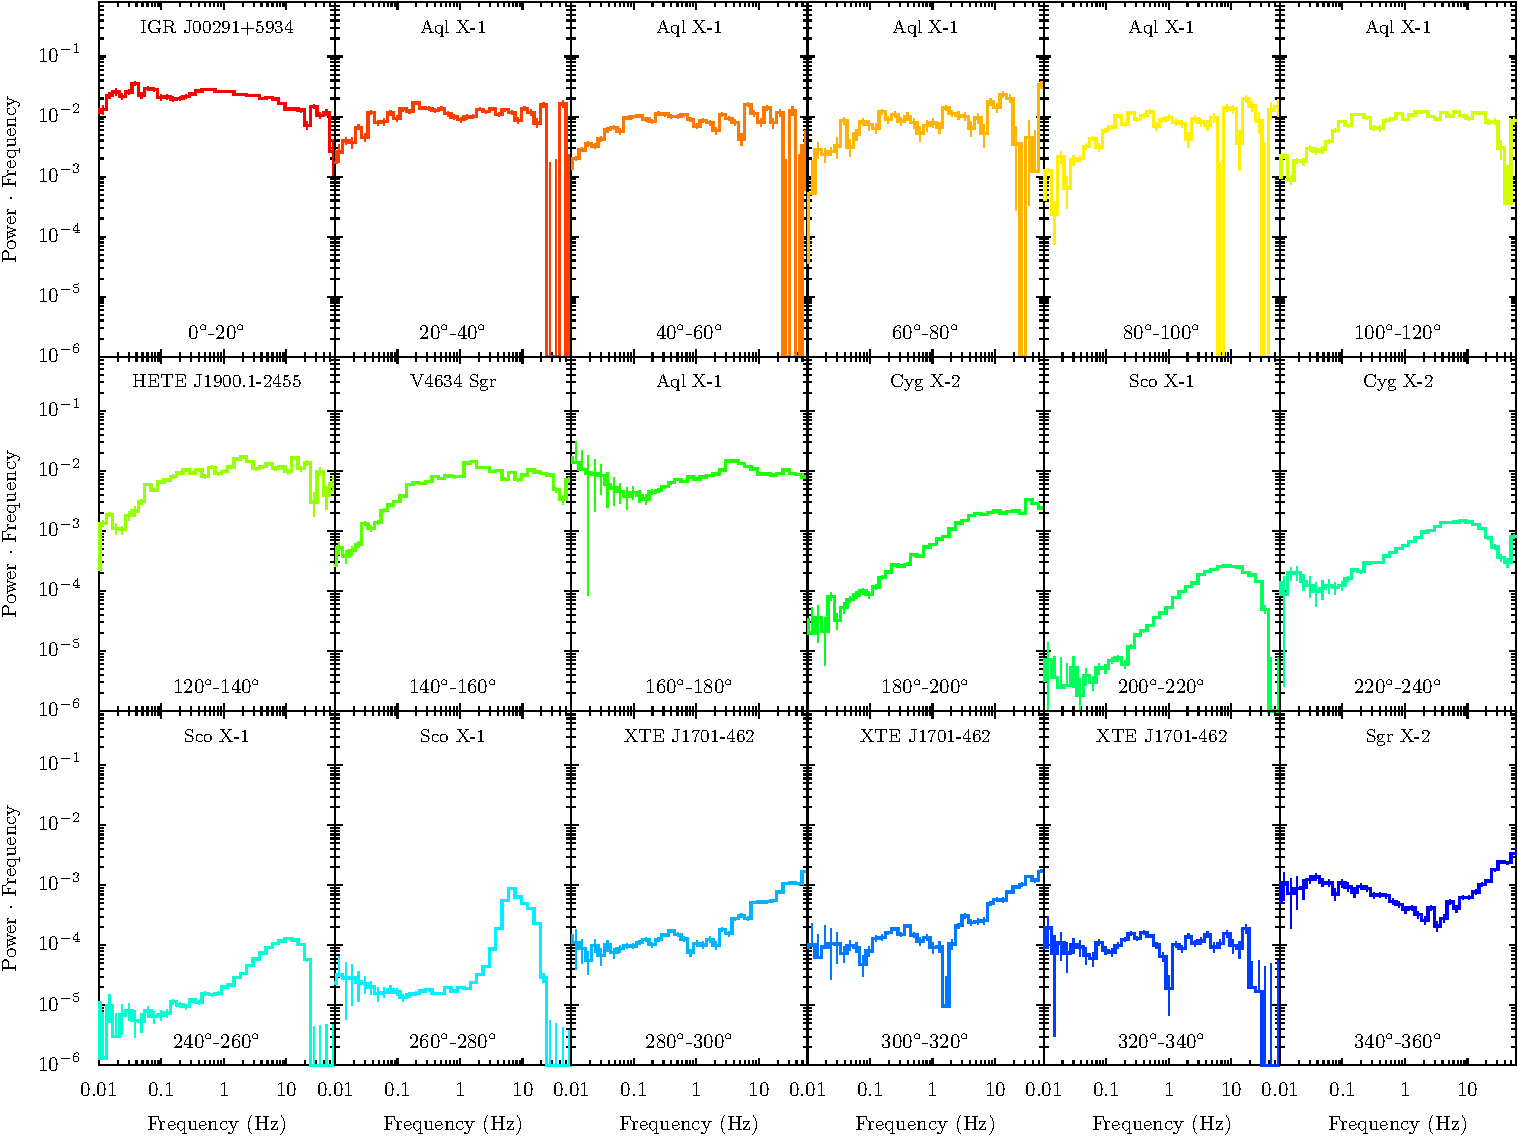
\includegraphics[width=0.9\linewidth]{ps/overview}}
%	\caption[Overview power spectra]{An overview with examples of neutron star power spectra per hue bin. Fig. \ref{fig:pc_hue_bins} shows this division in the \ac{PCC}~diagram. Each power spectrum represents a random power spectrum from the source with the most observations in that hue bin. Appendix~\ref{ch:psds} contains additional information, showing a larger selection of power spectra per hue bin.}\label{fig:ps_overview}
%\end{figure}
%\end{landscape}